\documentclass{astroedu-lab}

\begin{document}

\pagestyle{plain}

\begin{problem}{\huge Радиотехническая работа 77\\\\Применение операционных\\\\усилителей\\\\Выполнил Жданов Елисей Б01-205}

\section{Оборудование:}

Макетная плата

Набор резисторов различных номиналов

Набор конденсаторов различных номиналов

Операционный усилитель УД608

Тестер операционных усилителей

Мультиметр для проверки компонент

Электронный осциллограф на печатной плате

Электронный генератор сигналов на печатной плате

\section{Задание}

\subsection{Инвертирующий усилитель}

\begin{figure}[!h]
	\centering
	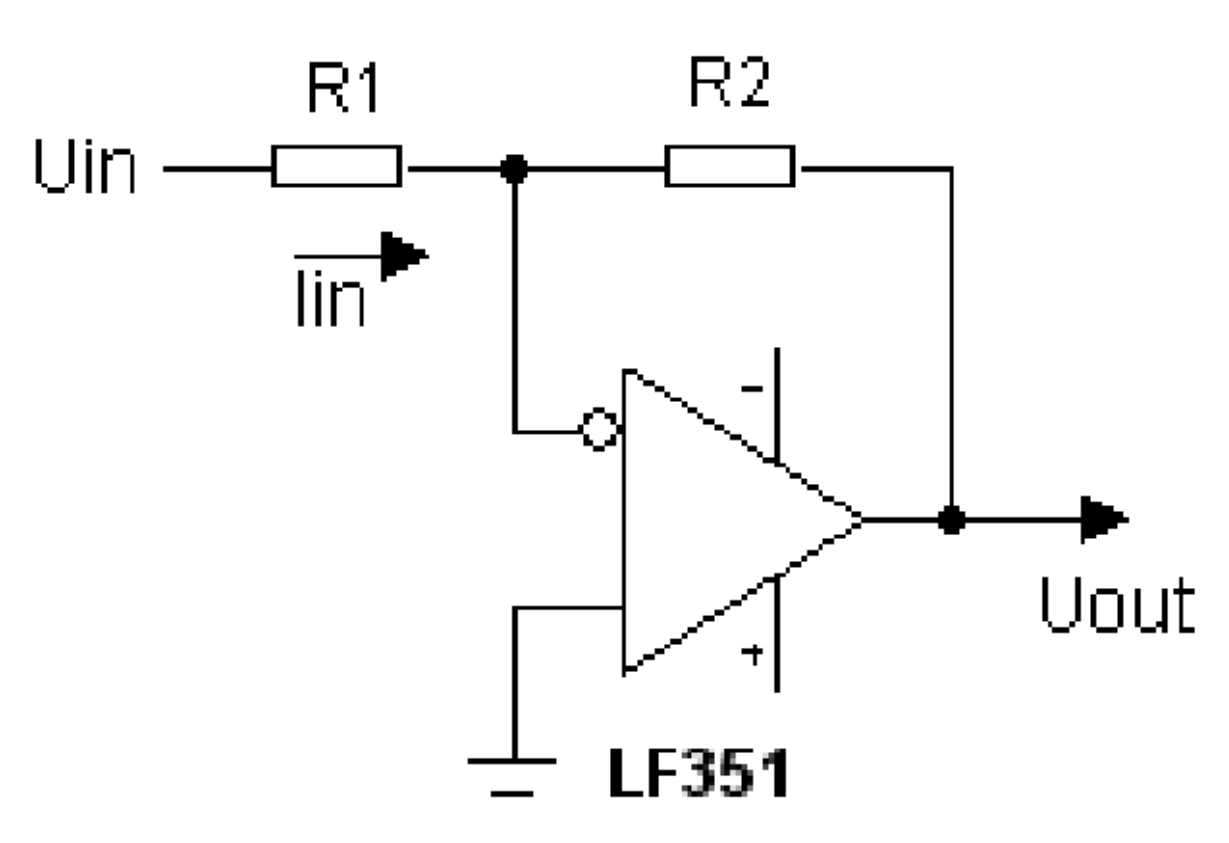
\includegraphics[width=0.5\textwidth]{invert.png}
	\label{fig:boiler}
\end{figure}

1) Соберем схему инвертирующего усилителя, используя $R = 1$ кОм, а $\frac{R_2}{R_1} = 200$.

2) Постоянное напряжение на выходе

$U_{out} = -0.1166$ В, напряжение сдвига $U_{os} = \frac{U_{out}}{200 + 1} = 0.6$ мВ.

3) Снимем зависимость $K(f)$ и построим граф Боде.

\begin{figure}[!h]
	\centering
	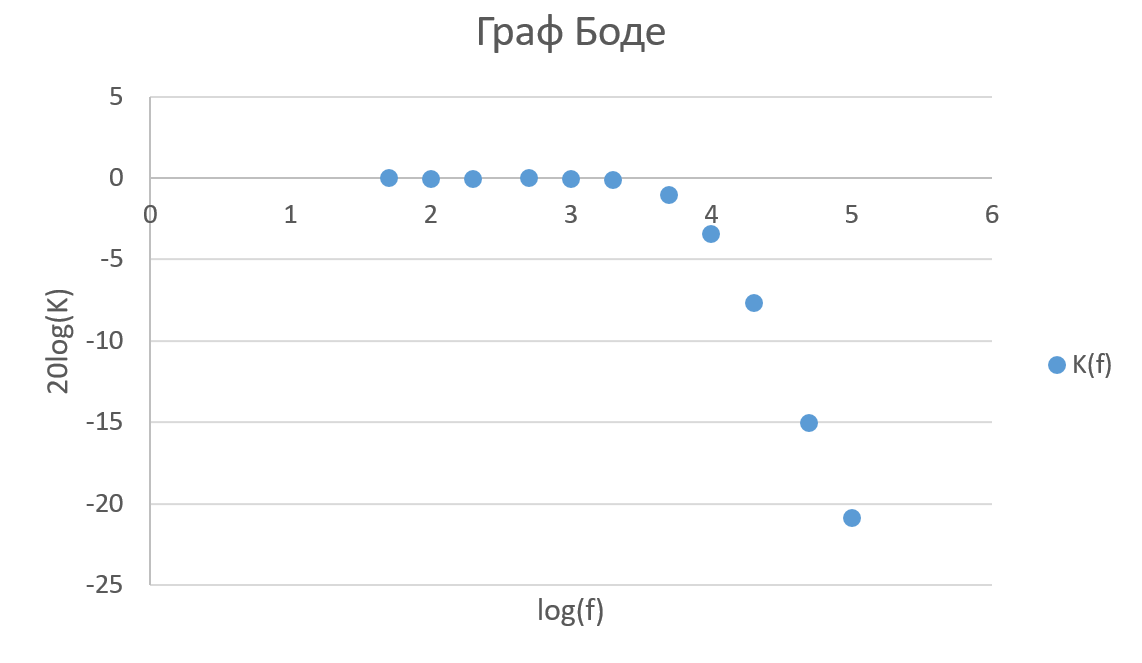
\includegraphics[width=0.9\textwidth]{bode.png}
	\label{fig:boiler}
\end{figure}

Граничная частота по уровню 0.7: $F_p = 800$ Гц.

5) На низкой частоте(1кГц - 2кГц) максимальная амплитуда неискаженного выходного сигнала составляет 0.075 В. Выше сигнал подвержен обычному клиппированию.

6) При включении ОУ по схеме повторителя ($R_1 = \infty, R_2 = 0$) коэффициент передачи единичный, максимальная амплитуда неискаженного сигнала $U = 4.5$ В, выше - клиппирование.

7) Замер напряжения на виртуальной земле показал значение $u = 4$ мВ при питании $e = 5$ мВ.

\subsection{Полосовой усилитель}

1) Соберем схему

\begin{figure}[!h]
	\centering
	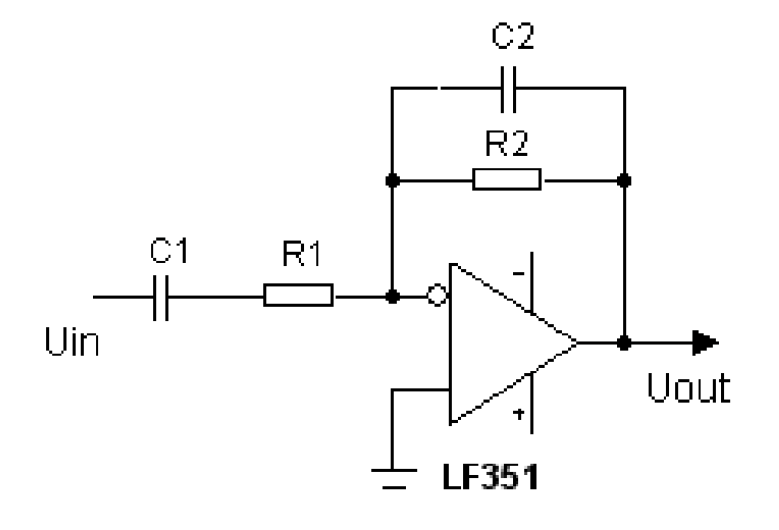
\includegraphics[width=0.5\textwidth]{band.png}
	\label{fig:boiler}
\end{figure}

с параметрами $R_1 C_1 = 10^{-3}$ сек и $R_2 C_2 = 10^{-5}$ сек, а также $\frac{R_2}{R_1} = 180$. Возьмем $R_1 = 1$ кОм, а $R_2 = 180$ кОм. Тогда $C_1 = 55$ нФ, а $C_1 = 1$ мкФ. 

Теоретические граничные частоты

\begin{equation}
	F_l = \frac{1}{2 \pi R_1 C_1} = 160 \text{ Гц}
\end{equation}

\begin{equation}
	F_2 = \frac{1}{2 \pi R_2 C_2} = 16 \text{ кГц}
\end{equation}

\begin{equation}
	F_0 = \sqrt{F_1 F_2} = 1.6 \text{ кГц}
\end{equation}

Линейный график

\begin{figure}[!h]
	\centering
	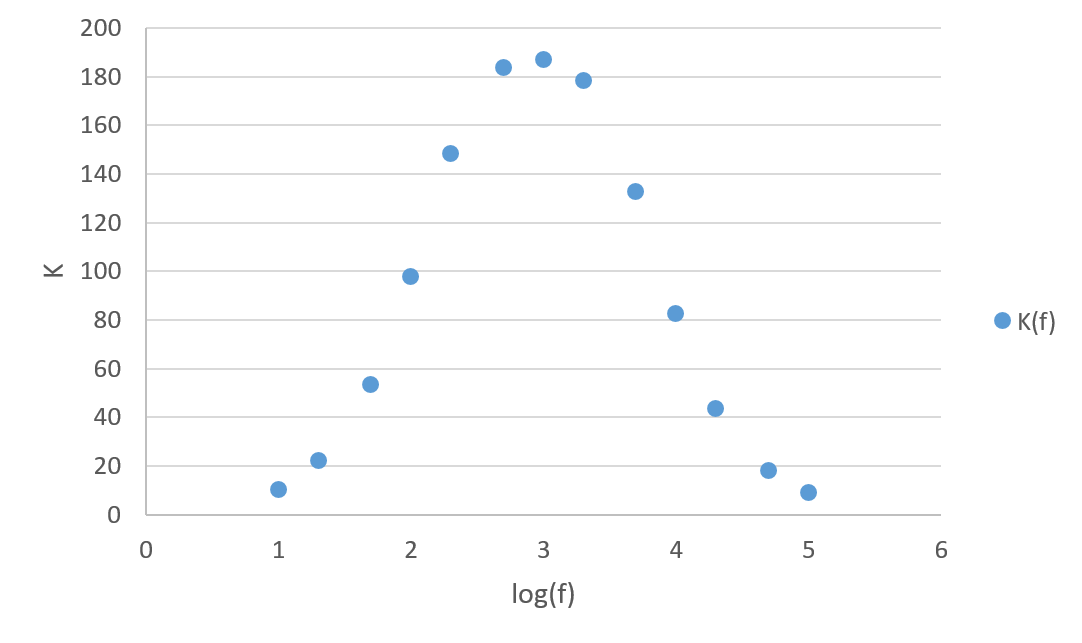
\includegraphics[width=0.9\textwidth]{bglin.png}
	\label{fig:boiler}
\end{figure}

Граф Боде

\begin{figure}[!h]
	\centering
	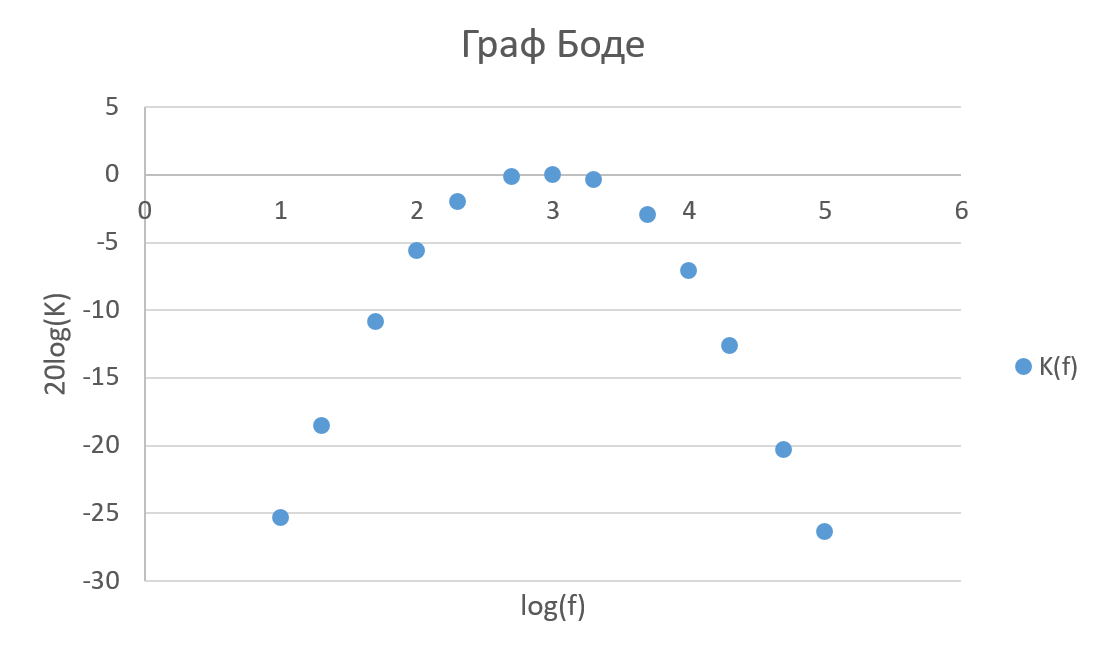
\includegraphics[width=0.9\textwidth]{bglog.png}
	\label{fig:boiler}
\end{figure}

Граничные частоты $F_1 = 146$ Гц и $F_2 = 14.9$ кГц.

Тогда частота максимума $F_{max} = 1470$ Гц, а напряжение $U = 6.797$ Вольт. $K_0 = 187$.

\subsection{Дифференциатор}

\begin{figure}[!h]
	\centering
	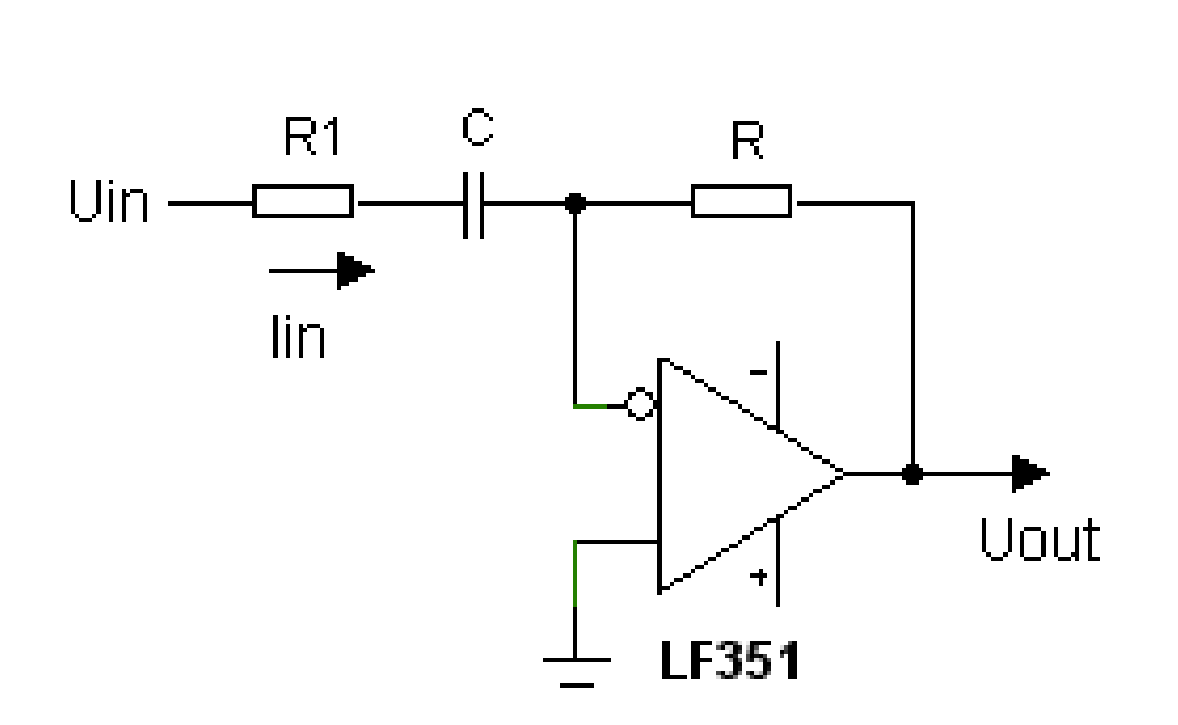
\includegraphics[width=0.5\textwidth]{dif.png}
	\label{fig:boiler}
\end{figure}

$\frac{R_2}{R_1} = 10$, $RC = 100 \text{ мс}$

АЧХ

\begin{figure}[!h]
	\centering
	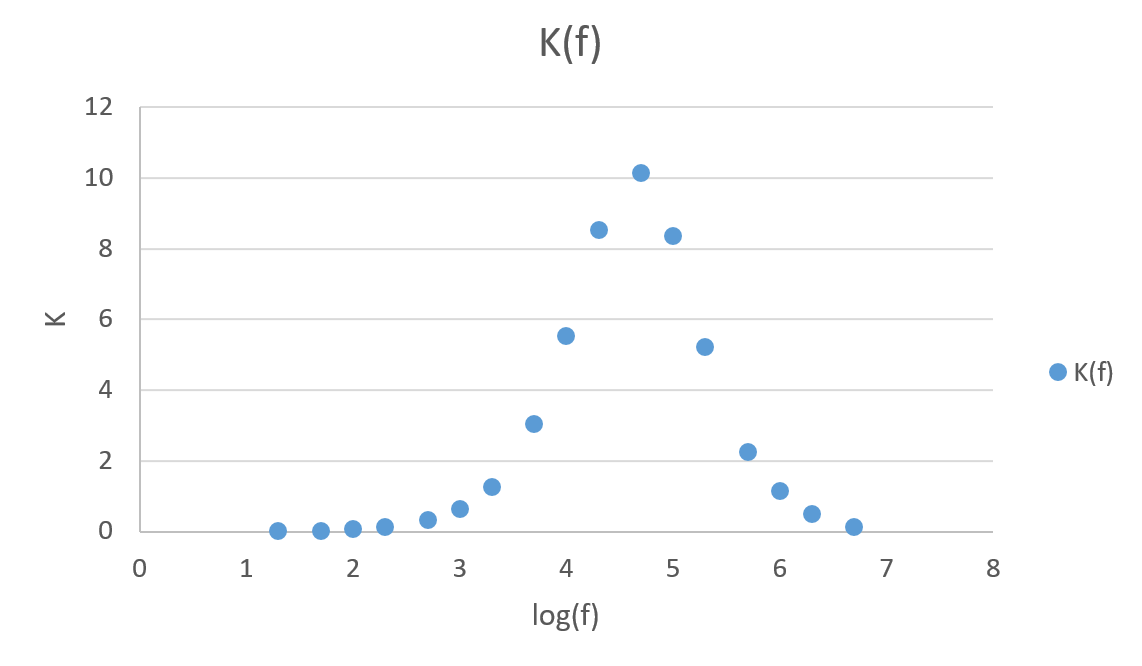
\includegraphics[width=0.9\textwidth]{difbd.png}
	\label{fig:boiler}
\end{figure}

\begin{figure}[!h]
	\centering
	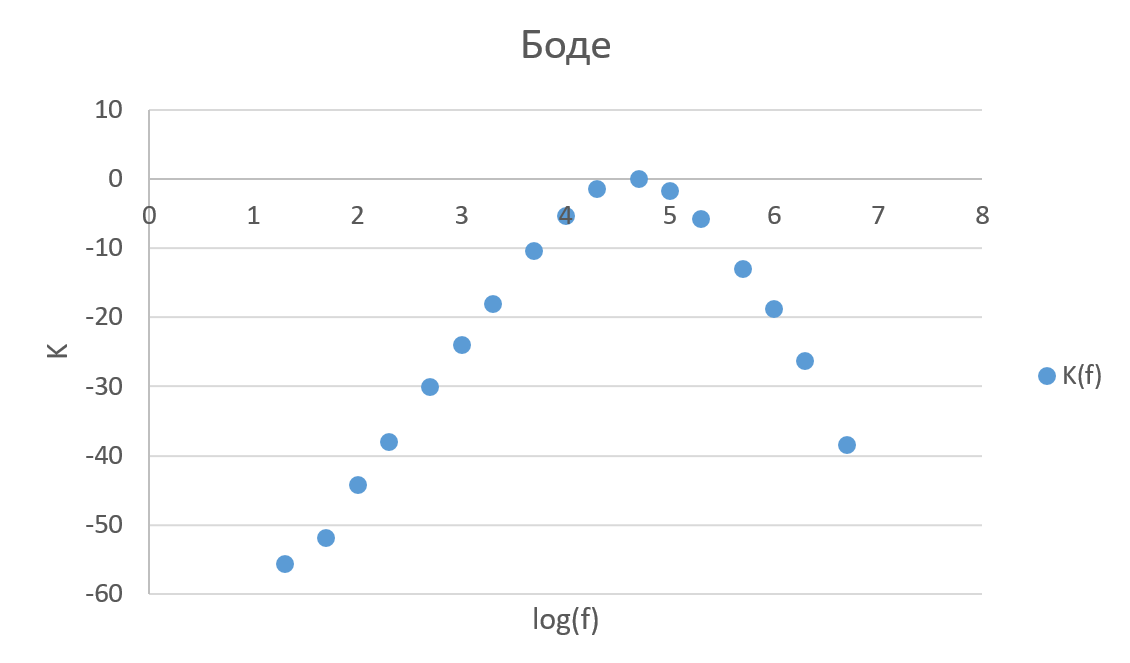
\includegraphics[width=0.9\textwidth]{diflog.png}
	\label{fig:boiler}
\end{figure}

Частоты единичного усиления 1.58 кГц и 1.14 МГц.

3) Подавая на вход треугольник и прямоугольник, получим соответствующие продифференцированные сигналы(прямоугольник со скачками).


%\subsubsection{Теория}
%
%В схеме делителя напряжения на рис. 16 напряжение $E$ идеального источника делится на части $U_1, U_2\left(U_1+U_2=E\right)$, падающие на резисторах $R_1, R_2$.
%
%Делитель - это распространенное схемное решение для преобразования источника питания $E$ в источник опорного напряжения с требуемым эквивалентным напряжением $E^*=E \frac{R_2}{R_1+R_2}$ и внутренним сопротивлением $R^*=\frac{R_1 R_2}{R_1+R_2}=R_1 \| R_2$, равным параллельному соединению сопротивлений $R_1, R_2$.
%
%Делитель естественным образом возникает, когда источник во внутренним сопротивлением $R_1$ подключается к нагрузке $R_2$, рис. 16 . Это сопровождается потерей уровня сигнала источника, выражаемой коэффициентом передачи $K=\frac{u}{e}=\frac{R_2}{R_1+R_2}$.
%
%\subsubsection{Выполнение}
%
%1. Соберем заданную схему на макетной плате. Подключим центральный узел схемы к измерительной ноге платы - генератора.
%
%Для схемы были выбраны резисторы $R_1$ = 3 кОм, а $R_2$ = 12 кОм(из пропорции $\frac{E-E^*}{R_1}=\frac{E^*}{R_2}$).
%
%Теоретически выбранное значение напряжения $E^*=2 \mathrm{~B}$, практически же  $E^*=2.056 \mathrm{~B}$. Различие действительно мало с учетом погрешности сопротивлений подобранных резисторов. Подаваемое значение напряжения питания $E=10 \mathrm{~B}$.
%
%%\begin{figure}[!h]
%%	\centering
%%	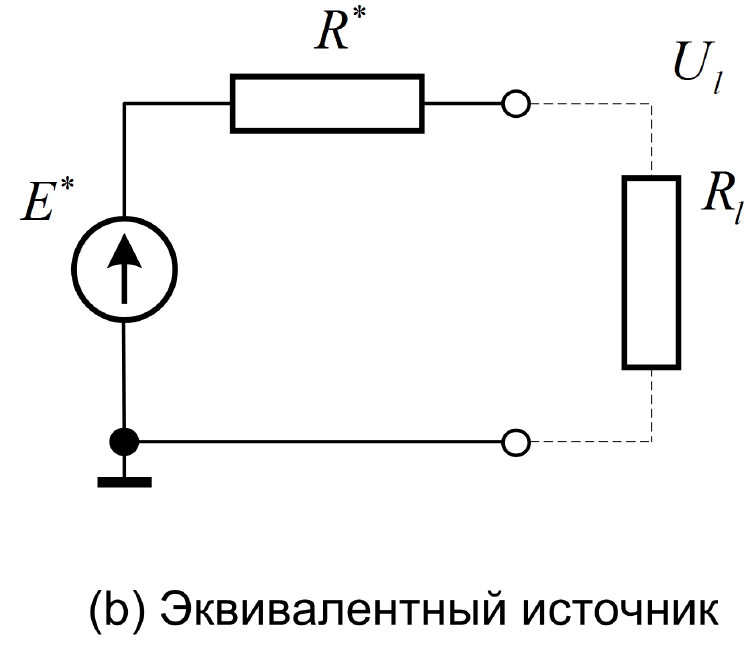
\includegraphics[width=0.32\textwidth]{16b.png}
%%	\label{fig:boiler}
%%\end{figure}
%
%Внутреннее сопротивление определим по методу двух нагрузок: измерим напряжение холостого хода на выходе делителя $U_{o c}=E^*=2.056 \mathrm{~B}$ и напряжение $U_l=0.9473 \mathrm{~B}$ на дополнительно подключенном резисторе нагрузки $R_l*=2$ кОм, см рисунок $16 \mathrm{b}$. Внутреннее сопротивление $R^*$ оценим из пропориции
%$$
%\frac{E^*-U_l}{R^*}=\frac{U_l}{R_l}
%$$
%
%Итого $R^*$ = 2.34 кОм. Теоретическое значение же равно $R^*$ = 2.4 кОм, что тоже довольно близко.
%
%%\begin{figure}[!h]
%%	\centering
%%	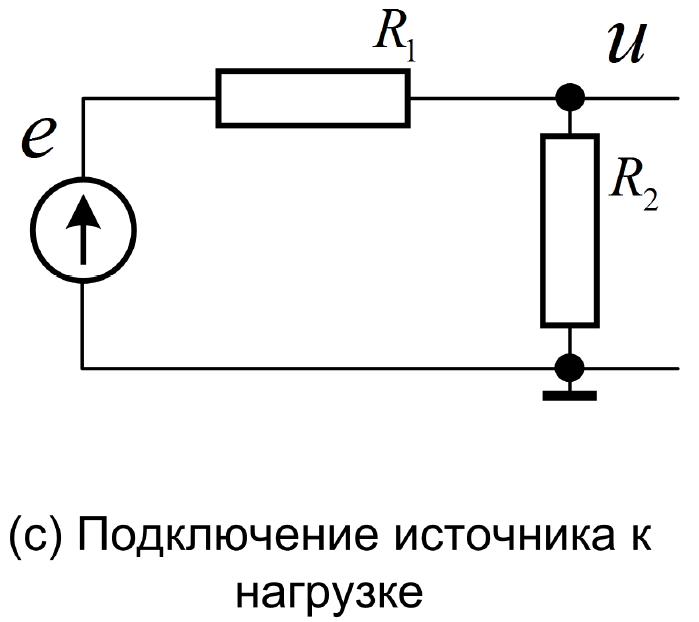
\includegraphics[width=0.3\textwidth]{16c.png}
%%	\label{fig:boiler}
%%\end{figure}
%
%2. Подадим а вход делителя синусоидальное напряжение $е = 1.02 \mathrm{~B}$ от лабораторного источника. На основании эффективного значения напряжения $u = 200.5 \text{ мВ}$, рассчитаю коэффициент передачи $K=\frac{u}{e} = 0.1966$, что почти равно теоретическому значению $K=\frac{u}{e} = 0.2$.
%
%\subsubsection{Вывод}
%
%Проведенные эксперименты подтверждают полученные теоретические выкладки. Разница между получаемыми теоретическими и практическими величинами почти постоянна и составляет около 2-3$\%$, что позволяет определить её как точность маркировки номиналов резисторов.
%
%\section{Вывод}
%
%Результаты моделирования, как и ожидается, тождественны теории, в то время как замеры на макетной плате незначительно от нее отличаются. Все это позволяет сказать, что использованные методы расчета и анализа безинерционных линейных цепей дают хорошие результаты в области применимости.


\end{problem}
\end{document}